\selectlanguage{italian}

\section{Nucleosintesi}

Le abbondanze relative degli elementi nell'Universo (Fig. \ref{iso-distr-univ}) sono correlate alle loro proprietà nucleari. Il processo di formazione di questi elementi è detto \textit{nucleosintesi}.

\subsection{Nucleosintesi del Big Bang}

Si stima che il primo evento di nucleosintesi risalga a $ \sim 3\,\text{min} $ dopo il Big Bang. In particolare, il primo secondo di vita dell'Universo dovrebbe essere stato caratterizzato da un equilibrio tra protoni e neutroni attraverso l'interazione debole:
\begin{equation*}
	n + e^+ \leftrightarrow p + \bar{\nu}_e
	\qquad
	p + e^- \leftrightarrow n + \nu_e
\end{equation*}
I successivi $ 3\,\text{min} $, invece, hanno visto il disaccoppiamento dei neutrini tramite i decadimenti $ \beta^{\pm} $ e la fotodissociazione del deuterio:
\begin{equation*}
	p + n \rightarrow \ch{^2 H} + \gamma \quad (Q = 2.2 \mev)
\end{equation*}
Per i successivi $ 17\,\text{min} $, lasso di tempo nel quale la temperatura dell'Univerto scese da $ T \sim 100 \kev $ a $ T \sim 10\kev $, i fotoni non ebbero più energia sufficiente per portare avanti la reazione di fotodissociazione, dunque le reazioni nucleari divennero efficaci. Questa è la \textit{Big Bang nucleosynthesis} (BBN), al termine della quale essenzialmente tutti i neutroni furono catturati in nuclei atomici: l'Universo a quel punto era composto da $ \ch{H} (75\%) $, $ \ch{He} (25\%) $ e tracce di $ \ch{Li} $ e $ \ch{Be} $.

\subsection{Nucleosintesi stellare}

Se la fonte di energia del Sole fosse esclusivamente la sua energia potenziale gravitazionale, dal teorema del viriale si avrebbe:
\begin{equation*}
	E = -\frac{1}{2} \Omega = - \frac{3}{4} \frac{GM_\odot^2}{R_\odot} \sim 3 \cdot 10^{41} \,\text{J}
	\quad \Rightarrow \quad
	\Delta t = \frac{E}{L_\odot} \sim 3 \cdot 10^{15} \,\text{s} = 24 \,\text{My}
\end{equation*}
Questa stima, però, è in disaccordo con l'età stimata della Terra $ \sim 4.5 \,\text{Gy} $. Negli anni 1920s si capì che la fonte energetica del Sole devono essere invece le reazioni di fusione nucleare: nonostante fosse noto che la temperatura del Sole non è abbastanza alta da permettere questo tipo di reazioni, a causa della barriera Coulombiana, il problema fu risolto da Gamow grazie all'effetto tunnel quantistico (idem alla sua teoria del decadimento $ \alpha $, si veda Sec. \ref{sec-gamow}). Negli anni successivi, Bethe e Weizsäcker studiarono i principali cicli di reazioni nel nucleo solare: la catena pp ed il ciclo CNO (Fig. \ref{sol-cyc}). In particolare, il ciclo CNO è responsabile delle tracce di elementi più pesanti presenti specialmente in stelle di seconda generazione (formate da gas espulso da esplosioni stellari) e diventa dominante alle alte temperature ($ \gtrsim 18 \,\text{MK} $ nel nucleo) a causa della barriera Coulombiana, specialmente in stelle più grandi del Sole: in quest'ultimo, solo l'1\% della produzione di energia è dovuta al ciclo CNO. La prova definitiva della nucleosintesi stellare avvenne con l'osservazione nel 1952 del tecnezio ($ T_{1/2} = 4.2 \,\text{My} $) nelle stelle, a dimostrazione della recente nucleosintesi.

\subsubsection{Bruciamento dell'idrogeno}

Il bruciamento dell'idrogeno avviene in stelle con $ T \gtrsim 10^7 \,\text{K} $ e $ M \gtrsim 0.08 M_\odot $. La principale reazione di fusione dell'idrogeno è:
\begin{equation*}
	4 \ch{^1 H} \rightarrow \ch{^4_2 He} + 2 e^+ + 2 \nu_e + 26.7\mev
\end{equation*}
Assumendo che tutta la produzione energetica solare sia dovuta a questa reazione, si possono calcolare il rate di fusione ed il tempo scala stimato per il bruciamento dell'idrogeno nel Sole:
\begin{equation*}
	N = \frac{L_\odot}{26.7\mev} \sim 10^{38} \,\text{s}^{-1}
	\quad \Rightarrow \quad
	M_{4\ch{^1 H}} = 4 m_p \cdot N \sim 6.4 10^{14} \,\text{g} \,\text{s}^{-1}
	\quad \Rightarrow \quad
	\Delta t = \frac{10\% M_\odot}{M_{4\ch{^1 H}}} \sim 10^{10} \,\text{y}
\end{equation*}
Questo valore è in accordo con l'età stimata della Terra.

\subsubsection{Bruciamento dell'elio}

Il bruciamento dell'elio avviene in stelle con $ T \gtrsim 10^8 \,\text{K} $ e $ M \gtrsim 0.4 M_\odot $, tipicamente a seguito della contrazione (e aumento della temperatura) dovuta al completo bruciamento del nucleo d'idrogeno, che a questo punto è un nucleo d'elio.\\
La fusione dell'elio è data da $ \ch{^4_2 He} + \ch{^4_2 He} \rightarrow \ch{^8_4 Be} $: quest'ultimo è un nuclide instabile che decade $ 2\alpha $ ($ T_{1/2} \sim 10^{-16}\,\text{s} $), dunque si viene a creare una concentrazione d'equilibrio (dinamico) di $ \ch{^8_2 Be} $. Inoltre, può avvenire un processo di cattura $ \ch{^8_4 Be} + \ch{^4_2 He} \rightarrow \ch{^{12}_6 C} $ in cui $ \ch{^{12}_6 C} $ ha un'energia prossima allo stato risonante a $ 7.656\mev $ e $ J^\pi = 0^+ $ detto \textit{stato di Hoyle}: questo stato si trova $ 285\kev $ al di sopra della configurazione $ \ch{^8 Be} + \alpha $ e decade principalmente $ \alpha $, sebbene abbia una bassa probabilità ($ \sim 0.04\% $) di decadere nel ground state. L'energia $ 285\kev $ corrisponde alla temperatura stellare $ \approx 2.5 \cdot 10^8 \,\text{K} $: il $ \ch{^{12} C} $ è un nucleo fortemente legato e fondamentale in quanto punto di partenza per la nucleosintesi di nuclei più pesanti.

\subsubsection{Stadi stellari avanzati}
\label{sec-stell-av}

Dopo bruciamento dell'$ \ch{He} $, la stella ha un nucleo di $ \ch{C} $ e $ \ch{O} $ (formato come $ \ch{^{12}C} \left( \alpha, \gamma \right) \ch{^{16}O} $, dunque la stella collassa e, se $ T \gtrsim 0.85 \cdot 10^9 \,\text{K} $ e $ M \gtrsim 8 M_\odot $, può innescare la combustione del carbonio, seguita dal bruciamento di neon e ossigeno (se $ T \gtrsim 1.5 \cdot 10^9 \,\text{K} $).\\
A seguito di ciò, gli elementi più abbondanti sono $ \ch{^{28}Si} $ e $ \ch{^{32}S} $: la barriera Coulombiana per la fusione di $ \ch{^{28}Si} $ è troppo alta, dunque diventa efficacie prima la fotodissociazione (se $ T \gtrsim 3 \cdot 10^9 \,\text{K} $): poiché non tutti i nuclei di $ \ch{^{28}Si} $ si dissociano, i rimanenti catturano le particelle leggere prodotte e formano nuclei più pesanti.\\
Le reazioni di fusione nucleare non procedono oltre il $ \ch{^{56}Fe} $, picco di stabilità per la average binding energy per nucleon, poiché il processo sarebbe endotermico: i nuclidi con $ A > 60 $ possono essere formati tramite cattura neutronica e successivo decadimento $ \beta $:
\begin{equation*}
	\ch{^A X} + n \rightarrow \ch{^{A+1} X} + \gamma
	\qquad
	\ch{^{A+1} X} \rightarrow \ch{^{A+1} Y} + e^- + \bar{\nu}_e
\end{equation*}
Detti $ \lambda_n $ e $ \lambda_\beta $ il tasso di cattura neutronica e di decadimento $ \beta $:
\begin{itemize}
	\item $ \lambda_n \ll \lambda_\beta $: il nucleo $ \ch{^{A+1} X} $ decade prima che ci sia tempo di catturare un secondo neutrone, poiché la cattura neutronica avviene con bassa frequenza e si parla di \textit{s-process} (slow);
	\item $ \lambda_n \gg \lambda_\beta $: sono possibili catture neutroniche multiple che spingono il nuclide sempre più lontano dalla valle di stabilità e si parla di \textit{r-process} (rapid).
\end{itemize}

\section{Esperimenti}

\subsection{Picco di Gamow}

Si consideri una reazione nucleare del tipo $ 0 + 1 \rightarrow 2 + 3 $. Il \textit{rate di reazione termonucleare} è definito come:
\begin{equation}
	r_{0,1} \defeq N_0 N_1 v \sigma(v)
	\label{eq:13.1}
\end{equation}
dove $ N_j $ è la densità numerica della $ j $-esima specie nucleare, $ v $ è la velocità relativa di $ 0 $ e $ 1 $ e $ \sigma(v) $ la sezione d'urto della reazione. $ r_{0,1} $ esprime un numero di reazioni per unità di tempo e di volume. Nelle stelle, le particelle sono in equilibrio termodinamico e seguono la distribuzione di Maxwell-Boltzmann:
\begin{equation}
	P(v) dv = \left( \frac{m_{0,1}}{2\pi k T} \right)^{3/2} e^{-m_{0,1} v^2 / 2kT} 4\pi v^2 dv
	\label{eq:13.2}
\end{equation}
Il rate di reazione termonucleare sarà quindi:
\begin{equation}
	r_{0,1} = N_0 N_1 \int_0^\infty v P(v) \sigma(v) dv \equiv N_0 N_1 \braket{\sigma v}_{0,1}
	\label{eq:13.3}
\end{equation}
Convertendo dalla velocità relativa all'energia del centro di massa:
\begin{equation*}
	P(E) dE = \frac{2}{\sqrt{\pi}} (kT)^{-3/2} \sqrt{E} e^{-E / kT} dE
	\quad \Rightarrow \quad
	\braket{\sigma v}_{0,1} = \sqrt{\frac{8}{\pi m_{0,1}}} (kT)^{-3/2} \int_0^\infty E \sigma(E) e^{-E / kT} dE
\end{equation*}
Detta $ E_c = Z_0 Z_1 \frac{e^2}{R} \sim 1 \mev $ il potenziale di repulsione Coulombiana, la sezione d'urto per $ E < E_c $ ha una dipendenza energetica $ \sim E^{-1} $. Inoltre, per effetto tunneling (analogo al decadimento $ \alpha $), si ha il coefficiente di trasmissione:
\begin{equation}
	\hat{T} \approx \exp \left[ - \frac{2\pi}{\hbar} \sqrt{\frac{m}{2E}} Z_0 Z_1 e^2 \right] \equiv e^{-2\pi \eta}
	\label{eq:13.4}
\end{equation}
La sezione d'urto è solitamente espressa come:
\begin{equation}
	\sigma(E) \equiv \frac{1}{E} e^{-2\pi \eta} S(E)
	\label{eq:13.5}
\end{equation}
dove $ S(E) $ è una funzione che varia lentamente con l'energia per una reazione non risonante, mettendo in risalto la forza d'interazione nucleare e gli effetti della struttura nucleare. Il rate di reazione termonucleare risulta essere dunque:
\begin{equation}
	r_{0,1} = \sqrt{\frac{8}{\pi m_{0,1}}} \frac{N_0 N_1}{(kT)^{3/2}} \int_0^\infty S(E) e^{-2\pi \eta} e^{-E/kT} dE
	\label{eq:13.6}
\end{equation}

\begin{figure}
	\centering
	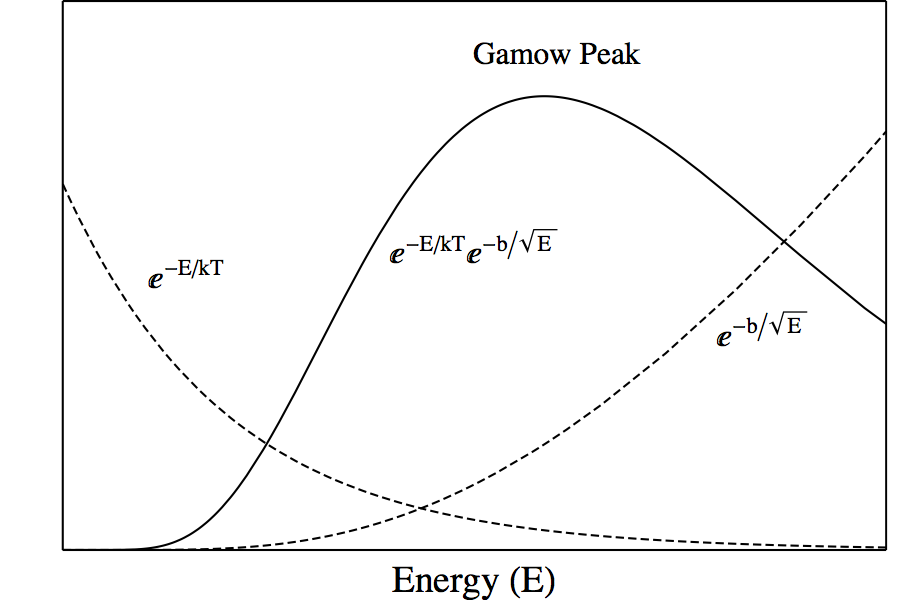
\includegraphics[width = 0.60 \textwidth]{gamow-peak.png}
	\caption{Gamow peak.}
	\label{gamow-peak}
\end{figure}

Fig. \ref{gamow-peak} mostra l'andamento di questa funzione dell'energia: risulta evidente che le reazioni avvengono efficaciemente soltanto in un certo intervallo di energie, detto \textit{picco di Gamow}. Si vede, inoltre, che la probabilità di tunneling diminuisce esponenzialmente al diminuire dell'energia, e con essa la sezione d'urto.

\subsection{Tecniche di laboratorio}

Un setup sperimentale tipico è costituito da:
\begin{enumerate}
	\item un accelleratore in grado di generare un fascio ad alta intensità e stabilità e con un basso spread di energia;
	\item un target ad elevata purezza e stabile sotto irraggiamento;
	\item un rilevatore con il miglior compromesso tra efficienza e risoluzione energetica, capace di rilevare prodotti di reazione tipici come $ \gamma $, $ p $, $ n $ ed $ \alpha $.
\end{enumerate}
Tipicamente, l'accelleratore è in grado di generare un flusso di proiettili $ N_p \sim 10^{14} \,\text{s}^{-1} $ (per correnti $ i \sim 0.1 \,\text{mA} $, il target (usually solid-state) presenta una densità di $ N_t \sim 10^{18} \,\text{cm}^{-2} $ e la sezione d'urto del processo è $ \sigma \sim 1 \,\text{pbarn} = 10^{-36}  \,\text{cm}^2 $, dunque, detta $ \varepsilon \in \left( 0.1 , 1 \right) $ l'efficienza del rilevatore, il rate di conteggi dell'esperimento è:
\begin{equation*}
	C = N_p N_t \sigma \varepsilon \sim 0.004 - 0.4 \,\text{h}^{-1}
\end{equation*}
Le principali sorgenti di rumore nelle misurazioni sono:
\begin{enumerate}
	\item radioattività ambientale: catene di $ \ch{^{235} U} $, $ \ch{^{238} U} $, $ \ch{^{232} Th} $ e $ \ch{^{40} K} $;
	\item raggi cosmici: principalmente muoni al livello del mare;
	\item neutroni: prodotti in reazioni $ \left( \alpha, n \right) $ e di spallazione.
\end{enumerate}
In particolare, i radioisotopi influiscono sulle misure a basse energie, mentre raggi cosmici e neutroni su quelle ad alte energie. Per migliorare il rapporto segnale/rumore, si può:
\begin{enumerate}
	\item aumentare il segnale: aumentando la corrente del fascio (ma degrada il target), aumentando la densità del bersaglio (ma il fascio perde energia ed avviene lo straggling) o migliorando l'efficienza del rilevatore;
	\item ridurre il fondo di rumore: con schermature attive o passive, con tecniche di soppressione del fondo o ponendo gli esperimenti underground.
\end{enumerate}
In particolare, i laboratori sotterranei costituiscono un ottimo metodo per ridurre il fondo di rumore, poiché le rocce riescono a sopprimere efficacemente il flusso di raggi cosmici. Rimane il problema dei radionuclidi, il quale può essere risolto prestando attenzione ai materiali scelti per la costruzione degli apparati (es.: piombo romano). L'Abruzzo ospita i più grandi laboratori sotterranei di fisica al mondo, i Laboratori Nazionali del Gran Sasso, con all'interno vari esperimenti: tra questi, l'esperimento LUNA (Laboratory for Underground Nuclear Astrophysics), che si occupa di studiare le reazioni attive in stelle massicce ed ambienti esplosivi.










